\documentclass[12pt,a4paper]{article}

\usepackage[T1]{fontenc}
\usepackage[utf8]{inputenc}
\usepackage{XCharter}
\usepackage[a4paper,left=10mm,right=10mm,top=11mm,bottom=15mm,footskip=8mm]{geometry}
\usepackage{array}
\usepackage{tabularx}
\usepackage{enumitem}
\usepackage{graphicx}
\usepackage{ragged2e}
\usepackage[normalem]{ulem}
\usepackage{microtype}
\usepackage{fancyhdr}
\usepackage{lastpage}
\usepackage[hidelinks,breaklinks=true]{hyperref}

\newif\ifwithphoto
\withphototrue

\hypersetup{
  pdftitle={Curriculum Vitae - Shengcheng Yu},
  pdfauthor={Shengcheng Yu},
  pdfsubject={Academic Curriculum Vitae}
}

\setlength{\parindent}{0pt}
\setlength{\parskip}{0pt}
\setlength{\tabcolsep}{0pt}
\setlength{\emergencystretch}{2em}
\raggedbottom
\urlstyle{same}

\pagestyle{fancy}
\fancyhf{}
\renewcommand{\headrulewidth}{0pt}
\renewcommand{\footrulewidth}{0pt}
\fancyfoot[C]{\fontsize{12}{14}\selectfont \thepage\ / \pageref*{LastPage}}

\newcommand{\cvsection}[1]{%
  \par\vspace{5pt}%
  \noindent\begin{minipage}{\linewidth}%
    \rule{\linewidth}{1.3pt}\par%
    \parbox[c][31pt][c]{\linewidth}{%
      \fontsize{20}{22}\selectfont\bfseries\itshape #1%
    }\par%
    \rule{\linewidth}{1.3pt}%
  \end{minipage}\par\nobreak\vspace{4pt}\nobreak%
}

\newcommand{\me}{\textbf{Shengcheng Yu}}
\newcommand{\cofirst}{\textsuperscript{\#}}
\newcommand{\corr}{\textsuperscript{*}}
\newcommand{\ccf}[1]{\textbf{[#1]}}
\newcommand{\awardtag}[1]{\textbf{\textit{\uline{#1}}}}

\newcommand{\publication}[5]{%
  \href{#5}{\textbf{\uline{#1}}}#2\par\nopagebreak[4]
  #3.\par\nopagebreak[4]
  #4\par\vspace{4.8pt}%
}

\newcommand{\funding}[4]{%
  \textbf{\uline{#1:}} \textbf{#2}#3\par
  #4\par\vspace{5pt}%
}

\newcommand{\summarytext}{%
  Postdoctoral Researcher at the Chair of Software Engineering \& AI, School of
  Computation, Information and Technology, Technical University of Munich (TUM),
  collaborating with Prof. Dr. Chunyang Chen. B.Eng. and Ph.D. degrees in Software
  Engineering obtained from Nanjing University in 2020 and 2024, supervised by
  Prof. Zhenyu Chen and Assoc. Prof. Chunrong Fang. Research interests span
  intelligent software testing, automated GUI testing, crowdsourced testing, GUI
  automation, human-agent collaboration, and LLM personification and personalization
  for software engineering.%
}

\begin{document}
\thispagestyle{fancy}

{\centering
  {\fontsize{30}{33}\selectfont\bfseries Dr. Shengcheng Yu}\par\vspace{7pt}
  \begin{tabular*}{\linewidth}{@{\extracolsep{\fill}}ccc@{}}
    \href{mailto:shengcheng.yu@tum.de}{\textbf{shengcheng.yu@tum.de}} &
    \href{mailto:yusc@nju.edu.cn}{\textbf{yusc@nju.edu.cn}} &
    \href{https://seysc.com}{\textbf{https://seysc.com}}
  \end{tabular*}\par
}

\ifwithphoto
  \vspace{8pt}
  \noindent
  \begin{minipage}[t]{0.775\linewidth}
    \fontsize{12}{17}\selectfont
    \justifying\summarytext
  \end{minipage}\hfill
  \begin{minipage}[t]{0.213\linewidth}
    \vspace{0pt}
    \raggedleft
    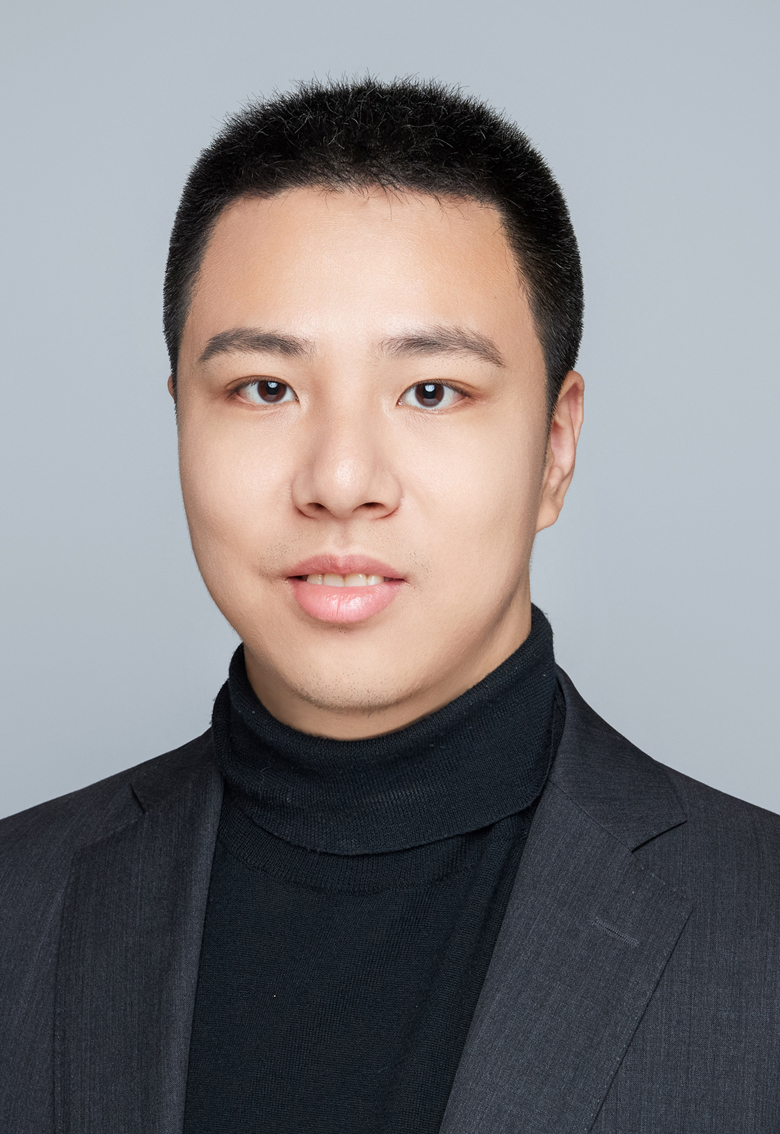
\includegraphics[width=114.08pt,height=164.94pt,keepaspectratio]{../YSC-CV.jpg}
  \end{minipage}
\else
  \vspace{-2pt}
  \cvsection{Summary}
  {\fontsize{12}{17}\selectfont
    \begin{itemize}[leftmargin=1.25em,label=\textbullet,topsep=0pt,itemsep=0pt,parsep=0pt]
      \item \justifying\summarytext
    \end{itemize}
  }
\fi

\cvsection{Experience}
\begingroup
\renewcommand{\arraystretch}{1.04}
\begin{tabular}{@{}>{\bfseries\raggedright\arraybackslash}m{0.42\linewidth}@{\hspace{8pt}}>{\itshape\raggedright\arraybackslash}m{0.33\linewidth}@{\hspace{8pt}}>{\raggedleft\arraybackslash}m{0.22\linewidth}@{}}
Technical University of Munich\newline School of Computation, Information and Technology & Postdoctoral Researcher & Feb. 2025 -- Now\tabularnewline[6pt]
Nanjing University\newline Software Institute & Research Assistant & Oct. 2024 -- Feb. 2025\tabularnewline[6pt]
Nanjing University\newline Software Institute & Ph.D.\newline in Software Engineering & Sep. 2020 -- Sep. 2024\tabularnewline[6pt]
ETH Zurich\newline Department of Computer Science & Visiting Ph.D.\newline in Software Engineering & Oct. 2022 -- Oct. 2023\tabularnewline[6pt]
Nanjing University\newline Software Institute & B.Eng.\newline in Software Engineering & Sep. 2016 -- Jun. 2020
\end{tabular}
\endgroup

\cvsection{Publication {\normalfont\fontsize{9}{10}\selectfont (\#: Co-first Author \quad *: Corresponding Author)}}

\begin{center}
\fontsize{10}{12}\selectfont
\begin{tabular*}{0.82\linewidth}{@{\extracolsep{\fill}}cccc@{}}
\textbf{Google Scholar Metrics:} &
\textbf{Citations:915} &
\textbf{h-index:15} &
\textbf{i10-index:21}
\end{tabular*}
\end{center}
\vspace{-4pt}
{\raggedleft\fontsize{9}{11}\selectfont\itshape @: as (co-)first author / corresponding author\par}
\vspace{3pt}

\begingroup
\fontsize{10}{14.4}\selectfont

\publication
{Software Engineering for and with GUI Agent}
{\ (Preprint)}
{\me, Yuchen Ling, Junyang Xing, Quan Zhou, Chunrong Fang\corr, Zhenyu Chen}
{}
{https://arxiv.org/abs/2608.09278}

\publication
{Toward Secure LLM Agents: Threat Surfaces, Attacks, Defenses, and Evaluation}
{\ (Preprint)}
{Yuchen Ling, \me\corr, Zhenyu Chen, Chunrong Fang\corr}
{}
{https://arxiv.org/abs/2606.10749}

\publication
{Mobile App Test Requirement Generation via Multimodal Information Fusion}
{}
{Peng Yang, Dayu Yang, \me, Yunfeng Zhu, Yong Tang\corr}
{\ccf{CCF-B} Journal of Systems and Software (JSS) 2026}
{https://doi.org/10.1016/j.jss.2026.113079}

\publication
{Bridging Stakeholder and Product Requirements: An Empirical Study of Requirement Engineering in the Automotive Industry}
{}
{Zixu Wang, \me\corr, Zhenchang Xing, Tobias Wenzel, Chunyang Chen}
{\ccf{CCF-A} IEEE/ACM International Conference on Automated Software Engineering (ASE) 2026 - Industry Showcase Track}
{https://doi.org/10.1145/3832783.3834456}

\publication
{More than a Judge: An Empirical Study of Agent-Human Interaction in Crowdsourced Testing Assessment}
{}
{Yue Wang, Yuan Zhao\corr, \me, Zhenyu Chen, Qing Gu}
{\ccf{CCF-A} ACM Transactions on Software Engineering and Methodology (TOSEM) 2026}
{https://doi.org/10.1145/3828168}

\publication
{Can Trajectory-Level Verdicts Be Trusted? An Empirical Study of Post-hoc Trajectory Interpretation for Mobile GUI Agents}
{\ (Accepted)}
{Yunfeng Zhu, \me, Zhenyu Chen\corr}
{\ccf{CCF-C} IEEE International Conference on Software Quality, Reliability, and Security (QRS) 2026}
{https://seysc.com}

\publication
{Scenario-Guided LLM-based Mobile App GUI Testing}
{}
{\me, Yuchen Ling, Chunrong Fang\corr, Quan Zhou, Yi Zhao, Chunyang Chen, Shaomin Zhu, Zhenyu Chen}
{\ccf{CCF-A} ACM Transactions on Software Engineering and Methodology (TOSEM) 2026. \textit{Accepted to present at ASE 2026 Journal-First Track}}
{https://doi.org/10.1145/3816025}

\publication
{Towards Automated Crowdsourced Testing via Personified-LLM}
{}
{\me, Yuchen Ling, Chunrong Fang, Zhenyu Chen, Chunyang Chen}
{\ccf{CCF-A} ACM International Conference on the Foundations of Software Engineering (FSE) 2026}
{https://doi.org/10.1145/3808173}

\publication
{Large Language Models for Software Testing Education: an Experience Report}
{}
{Peng Yang, Yunfeng Zhu, Chao Chang, \me, Zhenyu Chen, Yong Tang\corr}
{\ccf{CCF-A} ACM International Conference on the Foundations of Software Engineering (FSE) 2026 - Software Engineering Education Track}
{https://doi.org/10.1145/3803437.3805782}

\publication
{Software Testing Education Innovation for the Domestic Software and Hardware Ecosystem}
{}
{Zhenyu Chen, Chunrong Fang, \me, Jiawei Liu}
{Computer Education (in Chinese) 2026}
{http://doi.org/10.16512/j.cnki.jsjjy.2026.03.014}

\publication
{Survey on Application of Retrieval-augmented Generation in Software Engineering}
{}
{Quanjun Zhang, Chunrong Fang\corr, \me, Yuan Zhao, Zhenyu Chen}
{\ccf{CCF-A (Chinese)} Journal of Software (in Chinese) 2026}
{https://www.jos.org.cn/jos/article/abstract/7567}

\publication
{GUI Test Migration via LLM with Scenario-Granularity Understanding}
{}
{Quan Zhou, \me, Chunrong Fang\corr, Junyang Xing, Hongyi Yang, Jia Liu, Wenbin Guo, Zhenyu Chen}
{\ccf{CCF-B} Frontiers of Computer Science (FCS) 2026 - Letter}
{https://doi.org/10.1007/s11704-025-50270-x}

\publication
{A Survey on Large Language Models for Software Engineering}
{}
{Quanjun Zhang, Chunrong Fang, Yang Xie, Yaxin Zhang, \me, Weisong Sun, Yun Yang, Zhenyu Chen}
{\ccf{CCF-A} Science China Information Sciences (SCIS) 2026}
{https://doi.org/10.1007/s11432-025-4670-0}

\publication
{Human Cognitive Pattern Simulation for Crowdsourced Test Report Consistency Detection}
{}
{Yuchen Ling, \me, Shuguang Chen, Liuming Wang, Chunrong Fang\corr, Wenbin Guo, Jia Liu, Zhenyu Chen}
{\ccf{CCF-A} IEEE Transactions on Software Engineering (TSE) 2026}
{https://doi.org/10.1109/TSE.2026.3659293}

\publication
{Vision-Based Mobile App GUI Testing: A Survey}
{}
{\me, Chunrong Fang\corr, Ziyuan Tuo, Quanjun Zhang, Chunyang Chen, Zhenyu Chen, Zhendong Su}
{ACM Computing Surveys (CSUR) 2025}
{https://doi.org/10.1145/3773027}

\publication
{TestBench: Evaluating Class-Level Test Case Generation Capability of Large Language Models}
{}
{Quanjun Zhang, Ye Shang, Chunrong Fang\corr, Siqi Gu, \me, Jianyi Zhou, Zhenyu Chen\corr}
{\ccf{CCF-B} Frontiers of Computer Science (FCS) 2025}
{https://journal.hep.com.cn/fcs/EN/10.1007/s11704-025-50078-9}

\publication
{Multi-dimensional Assessment of Crowdsourced Testing Reports via LLMs}
{}
{Yue Wang, Yuan Zhao\corr, \me, Zhenyu Chen}
{\ccf{CCF-A} IEEE/ACM International Conference on Automated Software Engineering (ASE) 2025}
{https://doi.org/10.1109/ASE63991.2025.00150}

\publication
{LLM-based Crowdsourced Test Report Clustering}
{}
{Yue Wang, Yuan Zhao, \me, Zhenyu Chen}
{\ccf{CCF-A} ACM Transactions on Software Engineering and Methodology (TOSEM) 2025}
{https://doi.org/10.1145/3765756}

\publication
{Text--Image Fusion Template for Large Language Model Assisted Crowdsourcing Test Aggregation}
{}
{Yunfeng Zhu, \me, Zhaowei Zong, Yue Wang, Yuan Zhao\corr, Zhenyu Chen}
{\ccf{CCF-B} Journal of Systems and Software (JSS) 2025}
{https://doi.org/10.1016/j.jss.2025.112478}

\publication
{Test Script Intention Generation for Mobile Application via GUI Image and Code Understanding}
{}
{\me, Chunrong Fang\corr, Jia Liu\corr, Zhenyu Chen}
{\ccf{CCF-A} ACM Transactions on Software Engineering and Methodology (TOSEM) 2025}
{https://doi.org/10.1145/3722105}

\publication
{Semantic Matching-based Cross-Platform Mobile App Test Script Record and Replay via Large Language Models}
{}
{\me, Chunrong Fang\corr, Ye Zhong, Quanjun Zhang, Qin Liu, Jia Liu, Tao Zheng, Zhenyu Chen}
{\ccf{CCF-A (Chinese)} Journal of Software (in Chinese) 2025}
{https://www.jos.org.cn/jos/article/abstract/7414}

\publication
{Improving Retrieval-Augmented Deep Assertion Generation via Joint Training}
{}
{Quanjun Zhang, Chunrong Fang\corr, Yi Zheng, Ruixiang Qian, \me, Yuan Zhao, Jianyi Zhou, Yun Yang, Tao Zheng, Zhenyu Chen}
{\ccf{CCF-A} IEEE Transactions on Software Engineering (TSE) 2025}
{https://doi.org/10.1109/TSE.2025.3545970}

\publication
{Enhanced Crowdsourced Test Report Prioritization via Image-and-Text Semantic Understanding and Feature Integration}
{}
{Chunrong Fang, \me\corr, Quanjun Zhang, Xin Li, Yulei Liu, Zhenyu Chen}
{\ccf{CCF-A} IEEE Transactions on Software Engineering (TSE) 2025}
{https://doi.org/10.1109/TSE.2024.3516372}

\publication
{Redefining Crowdsourced Test Report Prioritization: An Innovative Approach with Large Language Model}
{}
{Yuchen Ling, \me, Chunrong Fang\corr, Guobin Pan, Jun Wang, Jia Liu\corr}
{\ccf{CCF-B} Information and Software Technology (IST) 2024}
{https://doi.org/10.1016/j.infsof.2024.107629}

\publication
{Practical, Automated Scenario-based Mobile App Testing}
{}
{\me, Chunrong Fang\corr, Mingzhe Du, Zimin Ding, Zhenyu Chen, Zhendong Su}
{\ccf{CCF-A} IEEE Transactions on Software Engineering (TSE) 2024}
{https://doi.org/10.1109/TSE.2024.3414672}

\publication
{Effective, Platform-Independent GUI Testing via Image Embedding and Reinforcement Learning}
{}
{\me, Chunrong Fang\corr, Xin Li, Yuchen Ling, Zhenyu Chen, Zhendong Su}
{\ccf{CCF-A} ACM Transactions on Software Engineering and Methodology (TOSEM) 2024}
{https://doi.org/10.1145/3674728}

\publication
{Semi-Supervised Crowdsourced Test Report Clustering via Screenshot-Text Binding Rules}
{}
{\me, Chunrong Fang\corr, Quanjun Zhang, Mingzhe Du, Jia Liu\corr, Zhenyu Chen\corr}
{\ccf{CCF-A} ACM International Conference on the Foundations of Software Engineering (FSE) 2024}
{https://doi.org/10.1145/3660776}

\publication
{Practical Non-Intrusive GUI Exploration Testing with Visual-based Robotic Arms}
{}
{\me, Chunrong Fang\corr, Mingzhe Du, Yuchen Ling, Zhenyu Chen, Zhendong Su}
{\ccf{CCF-A} IEEE/ACM International Conference on Software Engineering (ICSE) 2024}
{https://doi.org/10.1145/3597503.3639161}

\publication
{LLM for Test Script Generation and Migration: Challenges, Capabilities, and Opportunities}
{}
{\me, Chunrong Fang\corr, Yuchen Ling, Chentian Wu, Zhenyu Chen}
{\ccf{CCF-C} IEEE International Conference on Software Quality, Reliability, and Security (QRS) 2023}
{https://doi.org/10.1109/QRS60937.2023.00029}

\publication
{Towards Effective Bug Reproduction for Mobile Applications}
{}
{Xin Li\cofirst, \me\cofirst, Lifan Sun, Yuexiao Liu, Chunrong Fang\corr}
{International Conference on Dependable Systems and Their Applications (DSA) 2023. \awardtag{Best Paper Award}}
{https://doi.org/10.1109/DSA59317.2023.00024}

\publication
{Mobile App Crowdsourced Test Report Consistency Detection via Deep Image-and-Text Fusion Understanding}
{}
{\me, Chunrong Fang\corr, Quanjun Zhang, Zhihao Cao, Yexiao Yun, Zhenfei Cao, Kai Mei, Zhenyu Chen}
{\ccf{CCF-A} IEEE Transactions on Software Engineering (TSE) 2023}
{https://doi.org/10.1109/TSE.2023.3285787}

\publication
{Test Report Generation for Android App Testing via Heterogeneous Data Analysis}
{}
{Chunrong Fang\cofirst\corr, \me\cofirst, Ting Su\corr, Jing Zhang, Yuanhan Tian, Yang Liu (Co-first Author)}
{\ccf{CCF-A} IEEE Transactions on Software Engineering (TSE) 2023}
{https://doi.org/10.1109/TSE.2023.3237247}

\publication
{Leveraging Android Automated Testing to Assist Crowdsourced Testing}
{}
{Xiuting Ge, \me, Chunrong Fang\corr, Qi Zhu, Zhihong Zhao}
{\ccf{CCF-A} IEEE Transactions on Software Engineering (TSE) 2023}
{https://doi.org/10.1109/TSE.2022.3216879}

\publication
{SemCluster: A Semi-Supervised Clustering Tool for Crowdsourced Test Reports with Deep Image Understanding}
{}
{Mingzhe Du, \me, Chunrong Fang\corr, Tongyu Li, Heyuan Zhang, Zhenyu Chen}
{\ccf{CCF-A} ACM Joint European Software Engineering Conference and Symposium on the Foundations of Software Engineering (ESEC/FSE) 2022 - Demonstrations Track}
{https://doi.org/10.1145/3540250.3558933}

\publication
{Test Case Prioritization Using Partial Attention}
{}
{Quanjun Zhang, Chunrong Fang\corr, Weisong Sun, \me, Yutao Xu, Yulei Liu}
{\ccf{CCF-B} Journal of Systems and Software (JSS) 2022}
{https://doi.org/10.1016/j.jss.2022.111419}

\publication
{UniRLTest: Universal Platform-Independent Testing with Reinforcement Learning via Image Understanding}
{}
{Ziqian Zhang, Yulei Liu, \me, Xin Li, Yexiao Yun, Chunrong Fang\corr, Zhenyu Chen}
{\ccf{CCF-A} ACM SIGSOFT International Symposium on Software Testing and Analysis (ISSTA) 2022 - Tool Demonstrations Track}
{https://doi.org/10.1145/3533767.3543292}

\publication
{Layout and Image Recognition Driving Cross-platform Automated Mobile Testing}
{}
{\me, Chunrong Fang\corr, Yexiao Yun, Yang Feng}
{\ccf{CCF-A} IEEE/ACM International Conference on Software Engineering (ICSE) 2021}
{https://doi.org/10.1109/ICSE43902.2021.00139}

\publication
{Prioritize Crowdsourced Test Reports via Deep Screenshot Understanding}
{}
{\me, Chunrong Fang\corr, Zhenfei Cao, Xu Wang, Tongyu Li, Zhenyu Chen}
{\ccf{CCF-A} IEEE/ACM International Conference on Software Engineering (ICSE) 2021}
{https://doi.org/10.1109/ICSE43902.2021.00090}

\publication
{STIFA: Crowdsourced Mobile Testing Report Selection Based on Text and Image Fusion Analysis}
{}
{Zhenfei Cao, Xu Wang, \me, Yexiao Yun, Chunrong Fang\corr}
{\ccf{CCF-A} IEEE/ACM International Conference on Automated Software Engineering (ASE) 2020 - Tool Demonstrations Track}
{https://doi.org/10.1145/3324884.3415300}

\publication
{FuRong: Fusing Report of Automated Android Testing on Multi-Devices}
{}
{Yuanhan Tian\cofirst, \me\cofirst, Chunrong Fang\corr, Peiyuan Li}
{\ccf{CCF-A} IEEE/ACM International Conference on Software Engineering (ICSE) 2020 - Demonstrations Track}
{https://doi.org/10.1145/3377812.3382138}

\publication
{LIRAT: Layout and Image Recognition Driving Automated Mobile Testing of Cross-Platform}
{}
{\me, Chunrong Fang\corr, Yang Feng, Wenyuan Zhao, Zhenyu Chen}
{\ccf{CCF-A} IEEE/ACM International Conference on Automated Software Engineering (ASE) 2019 - Demonstrations Track}
{https://doi.org/10.1109/ASE.2019.00103}

\publication
{Crowdsourced Report Generation via Bug Screenshot Understanding}
{}
{\me}
{\ccf{CCF-A} IEEE/ACM International Conference on Automated Software Engineering (ASE) 2019 - Student Research Competition Track. \awardtag{First Place Award (Undergraduate) Winner}}
{https://doi.org/10.1109/ASE.2019.00161}

\publication
{From Data Quality to Model Quality: an Exploratory Study on Deep Learning}
{}
{Tianxing He, \me, Ziyuan Wang\corr, Jieqiong Li, Zhenyu Chen\corr}
{\ccf{CCF-C} Asia-Pacific Symposium on Internetware (Internetware) 2019}
{https://doi.org/10.1145/3361242.3361260}

\publication
{An Exploratory Study on Judicial Image Quality Assessment Based on Deep Learning}
{}
{Qiqi Gu, Weilin Cai, \me, Zhenyu Chen}
{\ccf{CCF-C} IEEE International Conference on Software Quality, Reliability, and Security (QRS) 2019}
{https://doi.org/10.1109/QRS.2019.00046}

\endgroup

\cvsection{Award}
\begin{itemize}[leftmargin=1.25em,label=\textbullet,topsep=0pt,itemsep=2pt,parsep=0pt]
  \item 2026 Nanjing University Outstanding Ph.D. Dissertation
  \item 2025 ACM Certified Reviewer
  \item 2023 Nanjing University Dongliang Scholarship (Award of Excellence in Academic Achievements)
  \item 2023 Nanjing University Excellent Graduate Student Pacemaker
  \item 2023 Nanjing University Excellent Graduate Student Innovation Project
  \item 2021 National Scholarship for Graduate Students
  \item 2021 Nanjing University Excellent Graduate Student Pacemaker
  \item 2021 College Student Innovation Annual Conference Elected Project of Ministry of Education
  \item 2020 Nanjing University - HPI Research Scholarship
  \item 2020 Nanjing University President's Special Scholarship for Ph.D. Student
  \item 2020 Nanjing University Outstanding Undergraduate Thesis - First Prize
  \item 2020 Nanjing University Software Institute Outstanding Graduate
  \item 2019 ACM SRC First Place Winner of Undergraduate Group in ASE 2019
  \item 2019 ACM SIGSOFT CAPS Program Award
\end{itemize}

\cvsection{Funding}
\funding{Principal Investigator}{Deutsche Forschungsgemeinschaft (DFG, German Research Foundation)}{ (583997361)}{KoQaGUI: Knowledge-Guided Quality Assurance of Software GUI}
\funding{Co-Principal Investigator}{ACM SIGSOFT Funding for Summer / Winter School}{}{LLM Software Development}
\funding{Key Participant}{National Key R\&D Program of China}{ (2024YFF0908000)}{Technology Research, Development, and Application of Open Source and Open Innovation Service Platform}
\funding{Principal Investigator}{Postgraduate Research \& Practice Innovation Program of Jiangsu Province}{ (KYCX22\_0174)}{Crowdsourced Test Report Optimization based on Multi-Modal Information Fusion Understanding}
\funding{Key Participant}{National Natural Science Foundation of China}{ (62141215)}{Crowdsourced Testing for Ubiquitous Operating System (UOS) Open Source Ecosystem}
\funding{Principal Investigator}{Nanjing University Training Program of Innovation for Undergraduates}{ (202010284073Z)}{Mobile Application Testing Research Based on Image Understanding}
\funding{Participant}{National Key R\&D Program of China}{ (2018YFB1403400)}{R\&D and Application of Integrated Crowdsourcing Test Service Platform for Information Products and Technology Services}
\funding{Participant}{National Natural Science Foundation of China}{ (61802171)}{Human-Machine Collaborative Mobile Application Testing Based on Comprehensible Information Fusion}

\cvsection{Teaching}
\begin{itemize}[leftmargin=1.25em,label=\textbullet,topsep=0pt,itemsep=2pt,parsep=0pt]
  \item \textbf{TUM: Seminar Automated Mobile App Testing (IN0014, IN2107, IN45110, INHN0015/\allowbreak INHN4010):} Lecturer (Summer / Winter 2025, 2026, 2027)
  \item \textbf{TUM: Development of LLM-driven GUI Agents (IN2106):} Lecturer (Summer 2025)
  \item \textbf{NJU: Automated Testing:} Teaching Assistant (2019, 2020, 2021, 2023, 2024)
  \item \textbf{NJU: Software Engineering and Computing III:} Teaching Assistant (2021, 2023)
  \item \textbf{NJU: Foundation of Computing System:} Teaching Assistant (2021)
\end{itemize}

\cvsection{Academic Service}
\begin{itemize}[leftmargin=1.25em,label=\textbullet,topsep=0pt,itemsep=1pt,parsep=0pt]
  \item \textbf{Conference Organizing Committee:}
    \begin{itemize}[leftmargin=1.25em,label=\textbullet,topsep=1pt,itemsep=1pt,parsep=0pt]
      \item LLM-Driven Software Testing Workshop (with ChinaSoft) (2026): Co-Chair
      \item UISE Workshop (with ICSE) (2026): Web \& Publicity Chair
    \end{itemize}
  \item \textbf{Journal Reviewer:}
    \begin{itemize}[leftmargin=1.25em,label=\textbullet,topsep=1pt,itemsep=1pt,parsep=0pt]
      \item ACM Transactions on Software Engineering and Methodology (TOSEM)
      \item IEEE Transactions on Software Engineering (TSE)
      \item IEEE Transactions on Dependable and Secure Computing (TDSC)
      \item Journal of Systems \& Software (JSS)
      \item Journal of Software: Evolution and Process
      \item Empirical Software Engineering (EMSE)
      \item International Journal of Human-Computer Interaction (IJHCI)
      \item IEEE Transactions on Reliability (TRel)
      \item IEEE Transactions on Intelligent Vehicles (TIV)
    \end{itemize}
  \item \textbf{Conference Technical/Research Track PC Member:}
    \begin{itemize}[leftmargin=1.25em,label=\textbullet,topsep=1pt,itemsep=1pt,parsep=0pt]
      \item International Conference on Software Engineering (ICSE): 2027 (also Shadow PC Area Chair)
      \item International Conference on the Foundations of Software Engineering (FSE): 2027
      \item IEEE/ACM International Conference on Automated Software Engineering (ASE): 2025, 2026
      \item ACM SIGSOFT International Symposium on Software Testing and Analysis (ISSTA): 2026
      \item International Joint Conferences on Artificial Intelligence (IJCAI): 2025, 2026
      \item IEEE International Conference on Software Maintenance and Evolution (ICSME): 2026
      \item ACM Conference on Intelligent User Interfaces (IUI): 2025, 2026, 2027
      \item Mining Software Repositories Conference (MSR): 2024, 2027
      \item International Workshop on Advances in Mobile App Analysis (A-Mobile): 2025
    \end{itemize}
  \item \textbf{Conference Artifact Evaluation Track PC Member:}
    \begin{itemize}[leftmargin=1.25em,label=\textbullet,topsep=1pt,itemsep=1pt,parsep=0pt]
      \item International Conference on Software Engineering (ICSE): 2024
      \item ACM SIGSOFT International Symposium on Software Testing and Analysis (ISSTA): 2024, 2025
    \end{itemize}
\end{itemize}

\cvsection{Invited Talk}
\begin{itemize}[leftmargin=1.25em,label=\textbullet,topsep=0pt,itemsep=2pt,parsep=0pt]
  \item \textbf{2025-06-18 \href{https://www.fortiss.org/}{Fortiss @ Munich}:} ``Intelligent GUI Testing with Knowledge Enhancement \& Persona-based AI''
  \item \textbf{2025-04-09 \href{https://ip.ai/}{IPAI @ Heilbronn}:} ``Beyond Chatbot: GUI Automation by LLM-based Agents''
\end{itemize}

\vspace{12pt}
\hfill\textbf{Last Updated: 2026-09-03}

\end{document}
